\documentclass{article}
\usepackage[utf8]{inputenc}
\usepackage{tikz}
\usetikzlibrary{shapes.geometric, arrows.meta, positioning}
\usepackage{geometry}
\geometry{a4paper, margin=1in}

\tikzstyle{criterion} = [rectangle, draw=black, fill=gray!20, rounded corners, text centered, text width=4cm, minimum height=1cm]
\tikzstyle{question} = [rectangle, draw=black, fill=blue!20, rounded corners, text centered, text width=7.5cm, minimum height=1.3cm]
\tikzstyle{example} = [rectangle, draw=black, fill=green!20, rounded corners, text centered, text width=16cm, minimum height=1.6cm]
\tikzstyle{arrow} = [thick,->,>=stealth]

\begin{document}

\begin{figure}[htp]
    \centering

    \label{fig:modern_slavery_flowchart}
    \hspace*{-2cm} % Adjust this value to shift the diagram to the left
    \scalebox{0.65}{ % Adjust the scaling factor to fit the page
    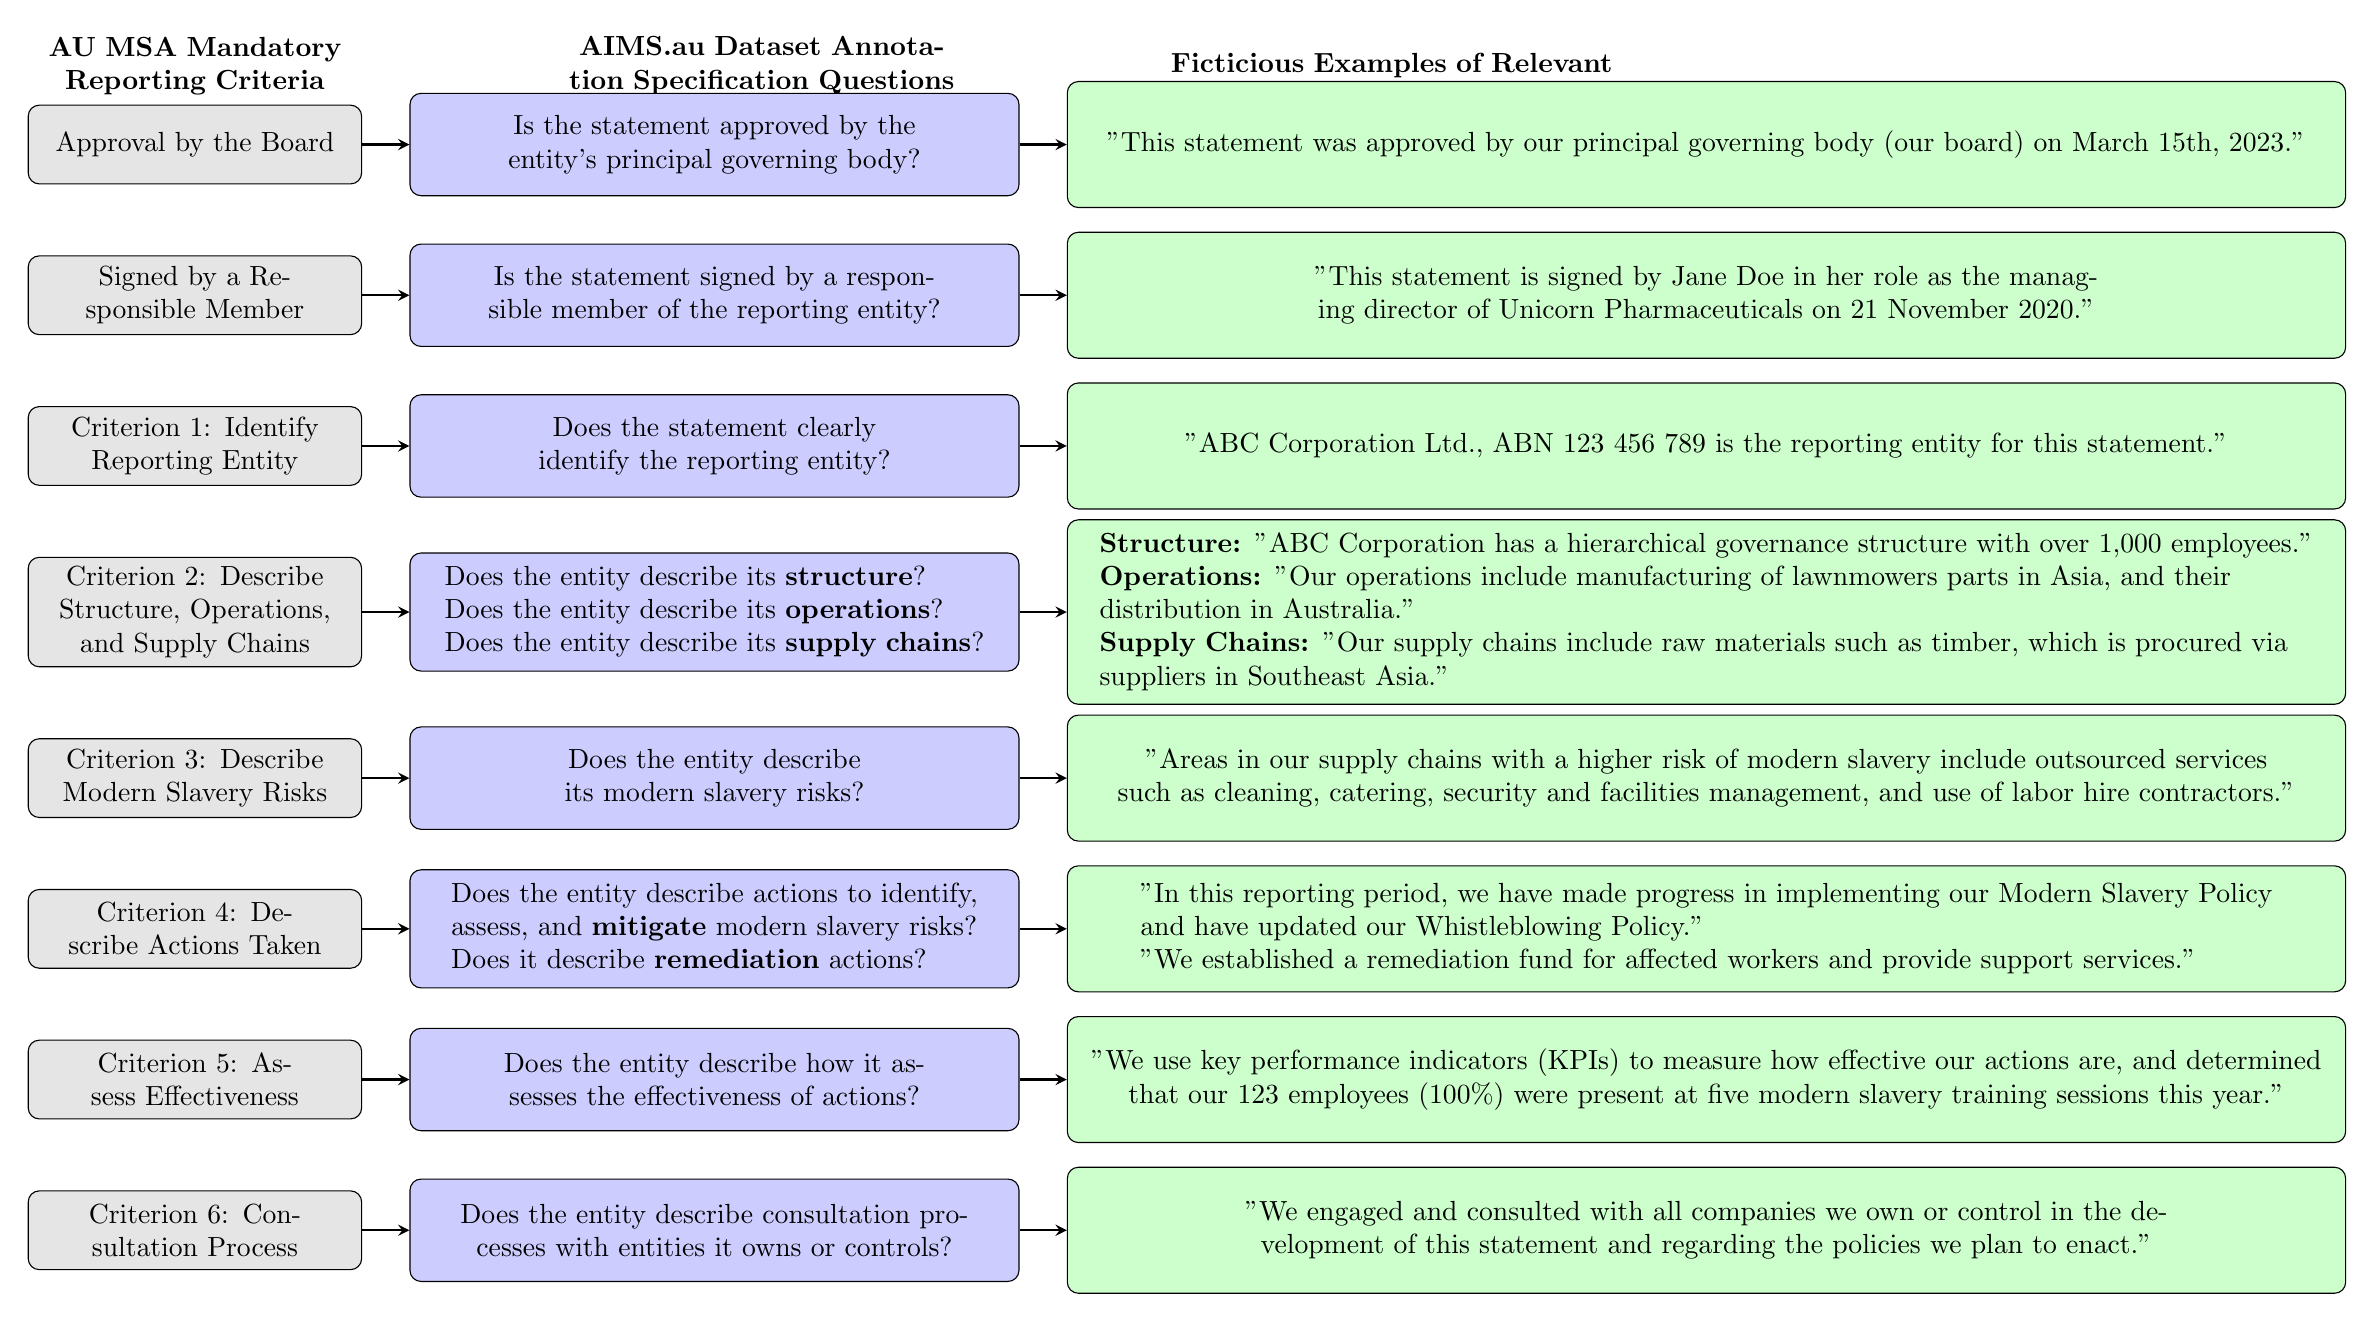
\begin{tikzpicture}[node distance=0.9cm and 0.6cm]

    % Column Labels
    \node[align=center, text width=4cm] (criterionLabel) at (-3.2, 1) {\textbf{AU MSA Mandatory Reporting Criteria}};
    \node[align=center, text width=7.5cm] (questionLabel) at (4, 1) {\textbf{AIMS.au Dataset Annotation Specification Questions}};
    \node[align=center, text width=13cm] (exampleLabel) at (12, 1) {\textbf{Ficticious Examples of Relevant}};

    % Approval and Signature Nodes
    \node[criterion] (approval) at (-3.2, 0) {Approval by the Board};
    \node[question, right=of approval] (approvalQuestion) {Is the statement approved by the entity’s principal governing body?};
    \node[example, right=of approvalQuestion] (approvalExample) {"This statement was approved by our principal governing body (our board) on March 15th, 2023."};

    \node[criterion, below=of approval] (signature) {Signed by a Responsible Member};
    \node[question, right=of signature] (signatureQuestion) {Is the statement signed by a responsible member of the reporting entity?};
    \node[example, right=of signatureQuestion] (signatureExample) {"This statement is signed by Jane Doe in her role as the managing director of Unicorn Pharmaceuticals on 21 November 2020."};

    % Criterion Nodes
    \node[criterion, below=of signature] (criterion1) {Criterion 1: Identify Reporting Entity};
    \node[question, right=of criterion1] (question1) {Does the statement clearly identify the reporting entity?};
    \node[example, right=of question1] (example1) {"ABC Corporation Ltd., ABN 123 456 789 is the reporting entity for this statement."};

    \node[criterion, below=of criterion1] (criterion2) {Criterion 2: Describe Structure, Operations, and Supply Chains};
    \node[question, right=of criterion2] (question2) {
        \begin{tabular}{l}
            Does the entity describe its \textbf{structure}?\\
            Does the entity describe its \textbf{operations}?\\
            Does the entity describe its \textbf{supply chains}?
        \end{tabular}
    };
    \node[example, right=of question2] (example2) {
        \begin{tabular}{l}
            \textbf{Structure:} "ABC Corporation has a hierarchical
            governance structure with over 1,000 employees."\\
            \textbf{Operations:} "Our operations include manufacturing of lawnmowers parts in Asia, and their  \\ distribution in Australia."\\
            \textbf{Supply Chains:} "Our supply chains include raw materials such as timber, which is procured via \\  suppliers in Southeast Asia."
        \end{tabular}
    };

    \node[criterion, below=of criterion2] (criterion3) {Criterion 3: Describe Modern Slavery Risks};
    \node[question, right=of criterion3] (question3) {Does the entity describe its modern slavery risks?};
    \node[example, right=of question3] (example3) {"Areas in our supply chains with a higher risk of modern slavery include outsourced services such as cleaning, catering, security and facilities management, and use of labor hire contractors."};

    \node[criterion, below=of criterion3] (criterion4) {Criterion 4: Describe Actions Taken};
    \node[question, right=of criterion4] (question4) {
        \begin{tabular}{l}
            Does the entity describe actions to identify,\\ assess,
            and \textbf{mitigate }modern slavery risks?\\
            Does it describe \textbf{remediation} actions?
        \end{tabular}
    };
    \node[example, right=of question4] (example4) {
        \begin{tabular}{l}
            "In this reporting period, we have made progress in implementing   our Modern Slavery Policy \\ and have updated our Whistleblowing Policy."\\
            "We established a remediation fund for affected workers and provide support services."
        \end{tabular}
    };

    \node[criterion, below=of criterion4] (criterion5) {Criterion 5: Assess Effectiveness};
    \node[question, right=of criterion5] (question5) {Does the entity describe how it assesses the effectiveness of actions?};
    \node[example, right=of question5] (example5) {"We use key performance indicators (KPIs) to measure how effective our actions are, and determined that our 123 employees (100\%) were present at five modern slavery training sessions this year."};

    \node[criterion, below=of criterion5] (criterion6) {Criterion 6: Consultation Process};
    \node[question, right=of criterion6] (question6) {Does the entity describe consultation processes with entities it owns or controls?};
    \node[example, right=of question6] (example6) {"We engaged and consulted with all companies we own or control in the development of this statement and regarding the policies we plan to enact."};

    % Arrows
    \draw[arrow] (approval.east) -- (approvalQuestion.west);
    \draw[arrow] (approvalQuestion.east) -- (approvalExample.west);

    \draw[arrow] (signature.east) -- (signatureQuestion.west);
    \draw[arrow] (signatureQuestion.east) -- (signatureExample.west);

    \draw[arrow] (criterion1.east) -- (question1.west);
    \draw[arrow] (question1.east) -- (example1.west);

    \draw[arrow] (criterion2.east) -- (question2.west);
    \draw[arrow] (question2.east) -- (example2.west);

    \draw[arrow] (criterion3.east) -- (question3.west);
    \draw[arrow] (question3.east) -- (example3.west);

    \draw[arrow] (criterion4.east) -- (question4.west);
    \draw[arrow] (question4.east) -- (example4.west);

    \draw[arrow] (criterion5.east) -- (question5.west);
    \draw[arrow] (question5.east) -- (example5.west);

    \draw[arrow] (criterion6.east) -- (question6.west);
    \draw[arrow] (question6.east) -- (example6.west);

    \end{tikzpicture}
    }

 \caption{Flowchart of Australian Modern Slavery Act Reporting Criteria}
\end{figure}

\end{document}
